\section{Arquitetura do sistema}

\subsection{Camadas}

O sistema está organizado em três camadas (Figura \ref{fig:arquitetura}). Na \textbf{camada de campo e controle}, o CLP lê os botões de Andon e os sensores da esteira e executa as máquinas de estados dos 12 postos. No \textbf{gateway de borda}, a Raspberry Pi consulta o CLP por Modbus RTU, guarda os eventos em uma fila SQLite durável, publica a telemetria por OPC UA, entrega os eventos de Andon por TCP e aciona o motor de passo da esteira pelos GPIOs. Na \textbf{supervisão}, o receptor no Windows persiste os eventos, assina a telemetria OPC UA e serve a Dashboard e a IT Digital E07 ao navegador.

\begin{figure}[H]
    \centering
    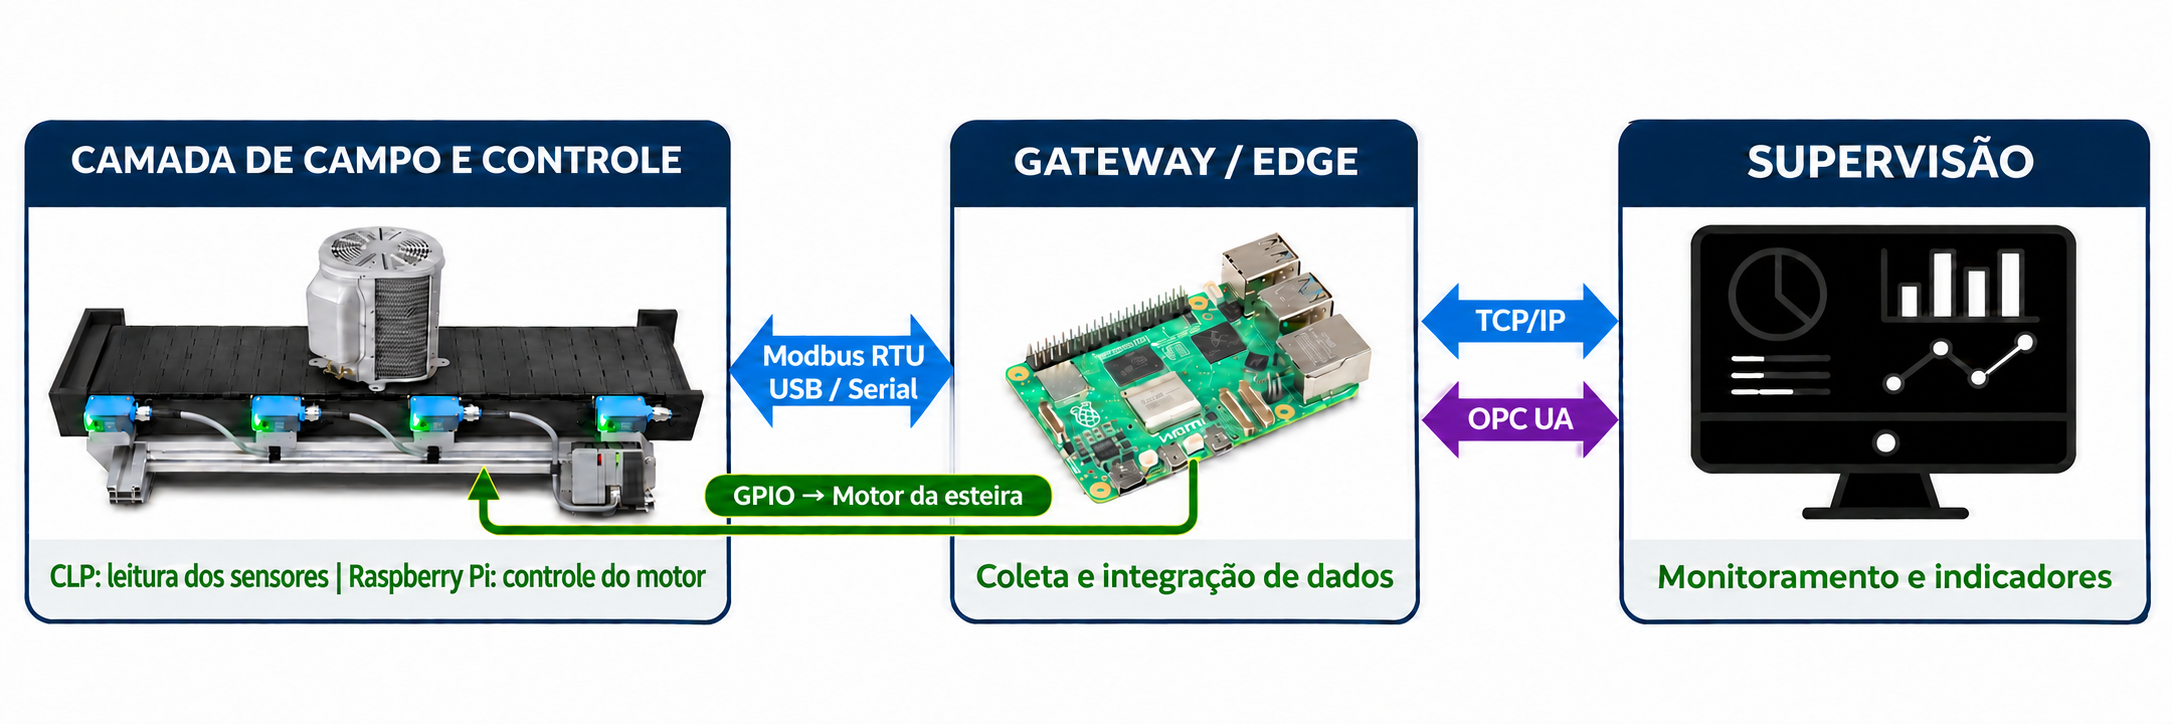
\includegraphics[width=1.00\textwidth]{Imagens/arquitetura_geral.png}
    \caption{Arquitetura em três camadas: campo e controle (CLP, sensores, esteira e motor), gateway de borda (Raspberry Pi) e supervisão (receptor e Dashboard no Windows). (arquivo: docs/Arquiteturas/Arquitetura.pptx)}
    \label{fig:arquitetura}
\end{figure}

\subsection{Enlaces e protocolos}

A Tabela \ref{tab:enlaces} lista os enlaces. A coluna ``Quem inicia'' indica o lado que abre a comunicação; as respostas retornam pelo mesmo enlace.

{\footnotesize
\begin{longtable}{|>{\centering\arraybackslash}p{0.6cm}|>{\raggedright\arraybackslash}p{3.0cm}|>{\raggedright\arraybackslash}p{3.0cm}|>{\raggedright\arraybackslash}p{2.2cm}|>{\raggedright\arraybackslash}p{6.2cm}|}
\caption{Matriz de enlaces da linha (portas do modelo de implantação \cod{hardware/deploy/config.raspberry.toml} e do receptor Windows).}\label{tab:enlaces}\\
\hline
\textbf{Nº} & \textbf{Quem inicia $\rightarrow$ destino} & \textbf{Protocolo} & \textbf{Porta / meio} & \textbf{O que trafega} \\ \hline
\endfirsthead
\hline
\textbf{Nº} & \textbf{Quem inicia $\rightarrow$ destino} & \textbf{Protocolo} & \textbf{Porta / meio} & \textbf{O que trafega} \\ \hline
\endhead
01 & Botões e sensores $\rightarrow$ CLP & Entradas digitais & Bornes de E/S & Níveis lógicos \cod{P00000}-\cod{P0000F} lidos pelo Ladder. \\ \hline
02 & Gateway $\rightarrow$ CLP & Modbus RTU (cliente/servidor) & RS-232 via adaptador USB-RS232, 115200 8N1, estação 1 & Leitura de estados, tempos, Andons, produção e eventos; escrita de ACK, relógio, base de tempos, Start e reset. \\ \hline
03 & Navegador $\rightarrow$ Windows & HTTP e WebSocket & TCP 8081 & Páginas, API REST e JSON em tempo real (\cod{/ws}, \cod{/ws/instruction/e07}). \\ \hline
04 & Gateway $\rightarrow$ receptor & Protocolo binário Andon sobre TCP & TCP 15000 & Evento de 16 bytes; o receptor devolve ACK ASCII de 22 bytes após persistir. \\ \hline
05 & Receptor $\rightarrow$ Gateway & OPC UA (\cod{opc.tcp}) & TCP 4840, \cod{/mock-linha/} & Assinatura de 74 variáveis e chamada de 6 métodos; \cod{Basic256Sha256} com \cod{SignAndEncrypt}. \\ \hline
06 & Gateway $\rightarrow$ servidor de hora & SNTP & UDP 123 & Hora de referência, convertida para \cod{America/Manaus} e gravada no relógio do CLP. \\ \hline
07 & Raspberry Pi $\rightarrow$ DRV8825 & GPIO & STEP BCM 18, DIR BCM 25, EN BCM 15 & Pulsos de passo, sentido e habilitação (EN ativo em nível baixo). \\ \hline
08 & DRV8825 $\rightarrow$ motor & Acionamento elétrico & Bobinas & Corrente controlada pelo driver. \\ \hline
\end{longtable}
}

\subsection{Fluxos principais}

\textbf{Entrega de um Andon.} (1) O operador aciona o botão; o Ladder grava oito palavras na FIFO \cod{D00300} e publica o evento em \cod{D00101}-\cod{D00108}, com a quantidade pendente em \cod{D00100}. (2) O Gateway lê o bloco por Modbus (FC04), grava os 16 bytes no SQLite com \cod{synchronous=FULL} e só então aciona \cod{P10000} (FC05). (3) O CLP retira o evento da fila. (4) O Gateway abre uma conexão TCP com o receptor e envia os 16 bytes; o receptor persiste e responde com o ACK de 22 bytes; só então o evento é marcado como confirmado. Os dois ACKs (\cod{P10000} e TCP) ocorrem em enlaces e momentos diferentes e garantem, respectivamente, que o Gateway guardou o evento e que o receptor o persistiu.

\textbf{Supervisão ao vivo.} O Gateway lê a cada 250 ms os Andons, Takt time, último ciclo, os 12 estados (\cod{D01651}-\cod{D01662}) e o contador de produção (\cod{D16052}) e publica as alterações no OPC UA. O receptor recebe as notificações por assinatura e a Dashboard envia o estado consolidado ao navegador a cada 1 s pelo WebSocket \cod{/ws}.

\textbf{Comandos do operador.} Os botões da Dashboard chamam a API HTTP do receptor, que chama métodos OPC UA do Gateway, que escreve no CLP por Modbus (Tabela \ref{tab:comandos}).

{\footnotesize
\begin{longtable}{|>{\raggedright\arraybackslash}p{2.0cm}|>{\raggedright\arraybackslash}p{3.6cm}|>{\raggedright\arraybackslash}p{3.6cm}|>{\raggedright\arraybackslash}p{5.6cm}|}
\caption{Caminho de cada comando do operador até o CLP.}\label{tab:comandos}\\
\hline
\textbf{Ação} & \textbf{Navegador $\rightarrow$ API} & \textbf{Receptor $\rightarrow$ Gateway (OPC UA)} & \textbf{Gateway $\rightarrow$ CLP (Modbus RTU)} \\ \hline
\endfirsthead
\hline
\textbf{Ação} & \textbf{Navegador $\rightarrow$ API} & \textbf{Receptor $\rightarrow$ Gateway (OPC UA)} & \textbf{Gateway $\rightarrow$ CLP (Modbus RTU)} \\ \hline
\endhead
Importar base & \cod{POST /api/process/cycle-base} & \cod{Linha/CarregarBaseCiclos} & FC16 grava 288 palavras em 12 blocos (\cod{D17001}-\cod{D17288}) e FC03 confere cada bloco. \\ \hline
Start & \cod{POST /api/process/start} & \cod{Linha/IniciarSimulacao} & FC05 pulsa \cod{P10002} por 2 s; a confirmação é um posto no estado 2. \\ \hline
Limpar base & \cod{POST /api/process/clear-base} & \cod{Linha/LimparBase} & FC05 pulsa \cod{P10003} por 2 s; o Gateway confere \cod{D16052 = 0}. \\ \hline
\end{longtable}
}
